% ======================================================================
\section{Entropic Randers affinities}
\label{sec:randers}

\subsection{Randers distances without a closed form}
\label{sec:approx}

The infimum \eqref{eq:dF} has no closed form when $\omega$ varies, and
computing it is impractical for neighbour embeddings, for three reasons
(\cref{app:randers}). Eikonal solvers for asymmetric metrics
\citep{sethian2003ordered,mirebeau2014efficient} need a grid, out of reach
in the $10$ to $50$ dimensions of single-cell data. Graph shortest paths
\citep{tenenbaum2000global} converge only as samples densify along the
optimal paths. Above all, $\omega$ is measured only at the samples,
$\omega_i=\omega(x_i)$, so the infimum over paths through empty regions
depends on an extension of $\omega$ that the data do not determine. We
therefore use costs built from the endpoint values only. With
$\Delta_{ij}=x_j-x_i$,
\begin{align}
  \dfr(x_i\to x_j)&=\|\Delta_{ij}\|+\omega_i^\top\Delta_{ij}
  &&\text{(frozen)},\label{eq:frozen}\\
  \dav(x_i\to x_j)&=\|\Delta_{ij}\|+\tfrac12(\omega_i+\omega_j)^\top\Delta_{ij}
  &&\text{(averaged)}.\label{eq:averaged}
\end{align}
Both are the length of the straight segment from $x_i$ to $x_j$, with the
drift integral replaced by a left-endpoint and a trapezoid rule. The
segment is not a geodesic in general, but it is close to one at short
range, and a kernel only weighs pairs at short range.

\begin{proposition}[Closed-form approximations]
  \label{prop:approx}
  Let $\omega\in C^2(\R^D)$ with $\sup\|\omega\|<1$, and let
  $L_1=\sup\|\nabla\omega\|$, $L_2=\sup\|\nabla^2\omega\|$ and
  $L_c=\sup\|\nabla\omega-\nabla\omega^\top\|$. For $r=\|y-x\|$:
  \begin{enumerate}
    \item $|\dfr(x\to y)-\ell(x,y)|\le\tfrac12L_1r^2$ and
      $|\dav(x\to y)-\ell(x,y)|\le\tfrac1{12}L_2r^3$, where $\ell$ is the
      Randers length of the straight segment;
    \item $0\le\ell(x,y)-\dF(x\to y)\le c\,L_c^2\,r^3$ whenever
      $L_cr\le c'$, for universal constants $c,c'$;
    \item if $\omega=\nabla\phi$, straight lines are geodesics and
      $\dF(x\to y)=\|y-x\|+\phi(y)-\phi(x)$.
  \end{enumerate}
  Hence $\dF-\dfr=O(L_1r^2)$ and $\dF-\dav=O\big((L_2+L_c^2)\,r^3\big)$.
\end{proposition}

Only the curl of $\omega$ makes bending the path worthwhile (item 2), and
for a gradient drift the averaged form is a trapezoid rule for the exact
$\phi(x_j)-\phi(x_i)$. Proofs are in \cref{app:randers}. On gradient
drifts in $D=50$, where $\dF$ is known exactly, the median relative error
over each point's $\sqrt n$ nearest neighbours is $1.5\times10^{-2}$
(frozen) against $1.1\times10^{-4}$ (averaged) for a convex potential,
and $2.3\times10^{-2}$ against $5.7\times10^{-3}$ for a non-convex one.
We use the averaged form throughout; it costs the same. It splits into a
symmetric part $S_{ij}=\|\Delta_{ij}\|$ and an antisymmetric one,
\begin{equation}
  \dav(x_i\to x_j)=S_{ij}+A_{ij},\qquad
  A_{ij}=\tfrac12(\omega_i+\omega_j)^\top\Delta_{ij},
  \label{eq:SA}
\end{equation}
where $A_{ij}=-A_{ji}$ is the work of the drift along the edge, an edge
flow on the complete graph. The frozen form has the same $A$.

\subsection{The affinity}
\label{sec:affinity}

\begin{definition}[Entropic Randers affinity]
  \label{def:era}
  Given samples $x_i$ and velocities $v_i$, let $\omega_i=-\rho\,v_i/\max_k\|v_k\|$
  with $\rho<1$ (default $0.95$), and $C_{ij}=\dav(x_i\to x_j)^q$
  (default $q=2$), $C_{ii}=+\infty$. Calibrate each row's bandwidth $\eps_i$
  by bisection so that the softmax of $-C_{i\cdot}/\eps_i$ has perplexity
  $\mathcal{P}$ (default $\sqrt n$). The \emph{row-stochastic} affinity
  $P^{\RS}$ is that softmax divided by $n$; the \emph{balanced} affinity
  $P^{\Sk}$ rescales the kernel $e^{-C_{ij}/\eps_i}$ to uniform marginals
  by Sinkhorn iterations.
\end{definition}

\begin{figure}[t]
  \centering
  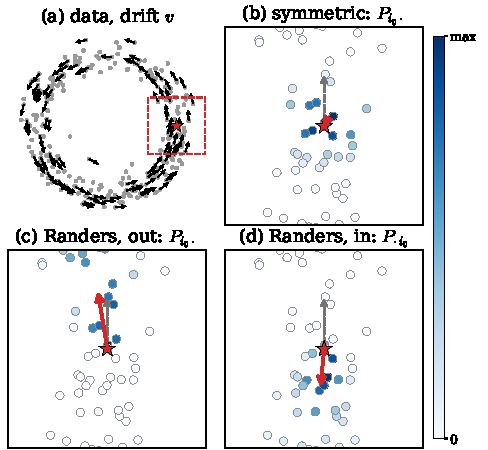
\includegraphics[width=\columnwidth]{figures/randers_affinity.pdf}
  \caption{Neighbourhood of one point $i_0$ ($\star$) on a rotating ring
  ($n=300$, \cref{def:era} with its defaults, balanced). (b--d) zoom on the
  dashed box of (a), one colour scale. Dashed grey: the velocity $v_{i_0}$;
  red: the affinity-weighted mean offset
  $\sum_jP_{ij}(x_j-x_{i_0})/\sum_jP_{ij}$, at true scale. The symmetric
  affinity is direction-blind (offset $0.006$). The Randers affinity sends
  mass downstream (row, offset $0.25$) and receives it from upstream
  (column, $0.17$).}
  \label{fig:randers_affinity}
\end{figure}

\Cref{fig:randers_affinity} shows the effect on a rotating ring: the row
of a point leans downstream, its column upstream. The global rescaling
keeps relative speeds, which a per-point normalisation of $v_i$ would
erase. The perplexity $\sqrt n$ keeps the
neighbourhood a fixed fraction of the data as $n$ grows; we found it
matters at scale (\cref{sec:implementation}). For $\omega=0$,
$P^{\Sk}$ is the balanced entropic affinity of SNEkhorn without the
symmetry constraint, and $P^{\RS}$ is the SNE affinity before
symmetrisation. Which of the two to use is not a detail: they keep
different parts of the drift.

\subsection{What normalisation keeps: a gauge}
\label{sec:gauge}

By \eqref{eq:scaling}, every normalisation adds to $-C/\eps$ a matrix of
the form $f_i+g_j$. Let $\Sep=\{(f_i+g_j)_{ij}:f,g\in\R^n\}$, let $\Asym$
be the antisymmetric matrices and
$\Grad=\{(\psi_j-\psi_i)_{ij}:\psi\in\R^n\}\subset\Asym$ the
\emph{gradient flows}. A short computation (\cref{app:proofs}) gives
$\Sep=\{(s_i+s_j)_{ij}\}\oplus\Grad$ and $\Sep\cap\Asym=\Grad$: the only
antisymmetric costs a rescaling can absorb are differences of a
potential.

\begin{theorem}[Identifiability modulo separable costs]
  \label{thm:identifiability}
  For fixed marginals and a global $\eps$, $\Sk(C)=\Sk(C')$ if and only if
  $C-C'\in\Sep$. In particular, for $C=S+A$ with $S$ symmetric and $A$
  antisymmetric, $\Sk(S+A)=\Sk(S+A')$ if and only if $A-A'\in\Grad$.
\end{theorem}

A balanced affinity thus sees the drift term $A$ only modulo gradients.
To say what remains, fix symmetric edge weights $W>0$ and define the
\emph{cyclic part} $\cyc_W(A)=A-\arg\min_{G\in\Grad}\sum_{ij}W_{ij}(A_{ij}-G_{ij})^2$,
the weighted Hodge projection of $A$ onto flows with no net $W$-flow out
of any point \citep{jiang2011statistical,lim2020hodge}. Then
$\cyc_W(A)=\cyc_W(A')$ if and only if $A-A'\in\Grad$, for every $W$:
the cyclic part is a complete invariant of what balancing sees. Its loop
sums are those of $A$, about $\oint\omega\cdot dx$ by Stokes' theorem:
the cyclic part is a discrete curl, or a flow around a hole of the
neighbourhood graph such as the cell cycle.

\begin{corollary}[Gradient drifts are pure gauge]
  \label{cor:gauge}
  Let $\omega=\nabla\phi$ and $C_{ij}=\|\Delta_{ij}\|+\phi(x_j)-\phi(x_i)$,
  the exact cost (\cref{prop:approx}). Then $\Sk(C)=\Sk(D)$ with
  $D_{ij}=\|\Delta_{ij}\|$. In particular a uniform drift $\omega\equiv c$,
  the gradient of $c^\top x$, is invisible to a balanced affinity.
\end{corollary}

The same holds for the mass that moves, for \emph{every} cost: if
$P\1=P^\top\1$, then $\sum_{ij}P_{ij}(f_j-f_i)=0$ for every $f\in\R^n$,
i.e.\ the net flow $P-P^\top$ has no divergence. A balanced affinity, and
every power of its Markov chain, makes no net progress along any
potential, a pseudotime for instance; it can only circulate.

\paragraph{Row-stochastic affinities keep the gradient part.}
For the same gradient cost, $\RS(C)_{ij}\propto e^{-D_{ij}/\eps}e^{-\phi(x_j)/\eps}$:
the symmetric affinity with targets reweighted towards low $\phi$, i.e.\
in the direction $-\omega$. For any $\alpha,\beta$ in \eqref{eq:scaling},
$\log(P_{ij}/P_{ji})=-2A_{ij}/\eps+\chi_j-\chi_i$ with
$\chi=\log\beta-\log\alpha$, so all normalisations share the cyclic part
of their log-asymmetry; they differ only in the gradient part $\chi$, set
by the marginals. $\RS$ leaves column sums free and records the gradient
part of the drift there; $\Sk$ prescribes them and removes it.

\paragraph{Leakage.}
Practical affinities break the gauge slightly. A squared cost
$(S+A)^2$ has the antisymmetric part $2S\odot A$, and per-row bandwidths
multiply row $i$ by $1/\eps_i$. Both multiply a gradient flow $G$
entrywise by a symmetric weight $m$, and since $c\,G\in\Grad$ for any
constant $c$,
\begin{equation}
  \|\cyc_W(m\odot G)\|_W\le\inf_c\|(m-c)\odot G\|_W .
  \label{eq:leak}
\end{equation}
In words: a gradient flow is invisible to balancing because it is the
difference of a potential, and multiplying it by a \emph{constant} keeps
it one. The squared cost and the row bandwidths instead multiply each
edge of the flow by its own weight, the edge's length and the bandwidth
of its row, and only the part of that weight that varies from edge to
edge, $m-c$, produces a flow that balancing can see. Where neighbour
distances and bandwidths are uniform, nothing leaks; where sampling
density varies, so do both, and a fraction of a gradient drift becomes
visible, in proportion to that variation and nowhere else. Perplexity
calibration, which adapts the bandwidth to the local density, is what
keeps $m$ close to constant in practice.
\todo[inline]{One or two numbers from experiments/theory/gauge\_checks (leak size at perplexity
$\sqrt n$, $q=2$) to show the attenuation is strong but not total.}

\paragraph{Which normalisation for which data.}
\Cref{fig:hodge} illustrates the split on a ring. For velocities
dominated by their gradient part, such as differentiation trajectories,
balancing discards most of the signal and the row-stochastic affinity
should be used. For circulating dynamics, such as the cell cycle,
balancing isolates the circulation and keeps the marginal control that
motivated SNEkhorn. A Hodge decomposition of the velocity on the
neighbourhood graph tells which regime a dataset is in. On mouse
gastrulation the gradient part carries 75--83\% of the velocity's edge
flow and all of its forward-in-time content; on RPE1 cell-cycle data the
progress around the cycle is carried by the cyclic part alone
(\cref{app:hodge_data}).

\begin{figure}[t]
  \centering
  \todo[inline]{Compact one-row version of the ring figure for the main text
  (graph cost: full / gradient / cyclic, and balanced $P_{ji}-P_{ij}$);
  the full four-row version is \cref{fig:hodge_full}.}
  \caption{Hodge split of a Randers drift on a ring, $\omega=$ rotation
  $+$ uniform drift, on a 5-NN graph. The gradient part is invisible to the
  balanced affinity, whose net transport is the cyclic part only; the
  row-stochastic affinity transports along both.}
  \label{fig:hodge}
\end{figure}
